\newpage
\subsection{Emitters}
\label{sec:emitters}
Mitsuba supports a wide range of emitters/light sources, which can be classified
into two main categories: emitters which are located somewhere within the scene, and emitters
that \emph{surround} the scene to simulate a distant environment. An overview of the available
types is shown below:
\begin{figure}[h!]
\centering
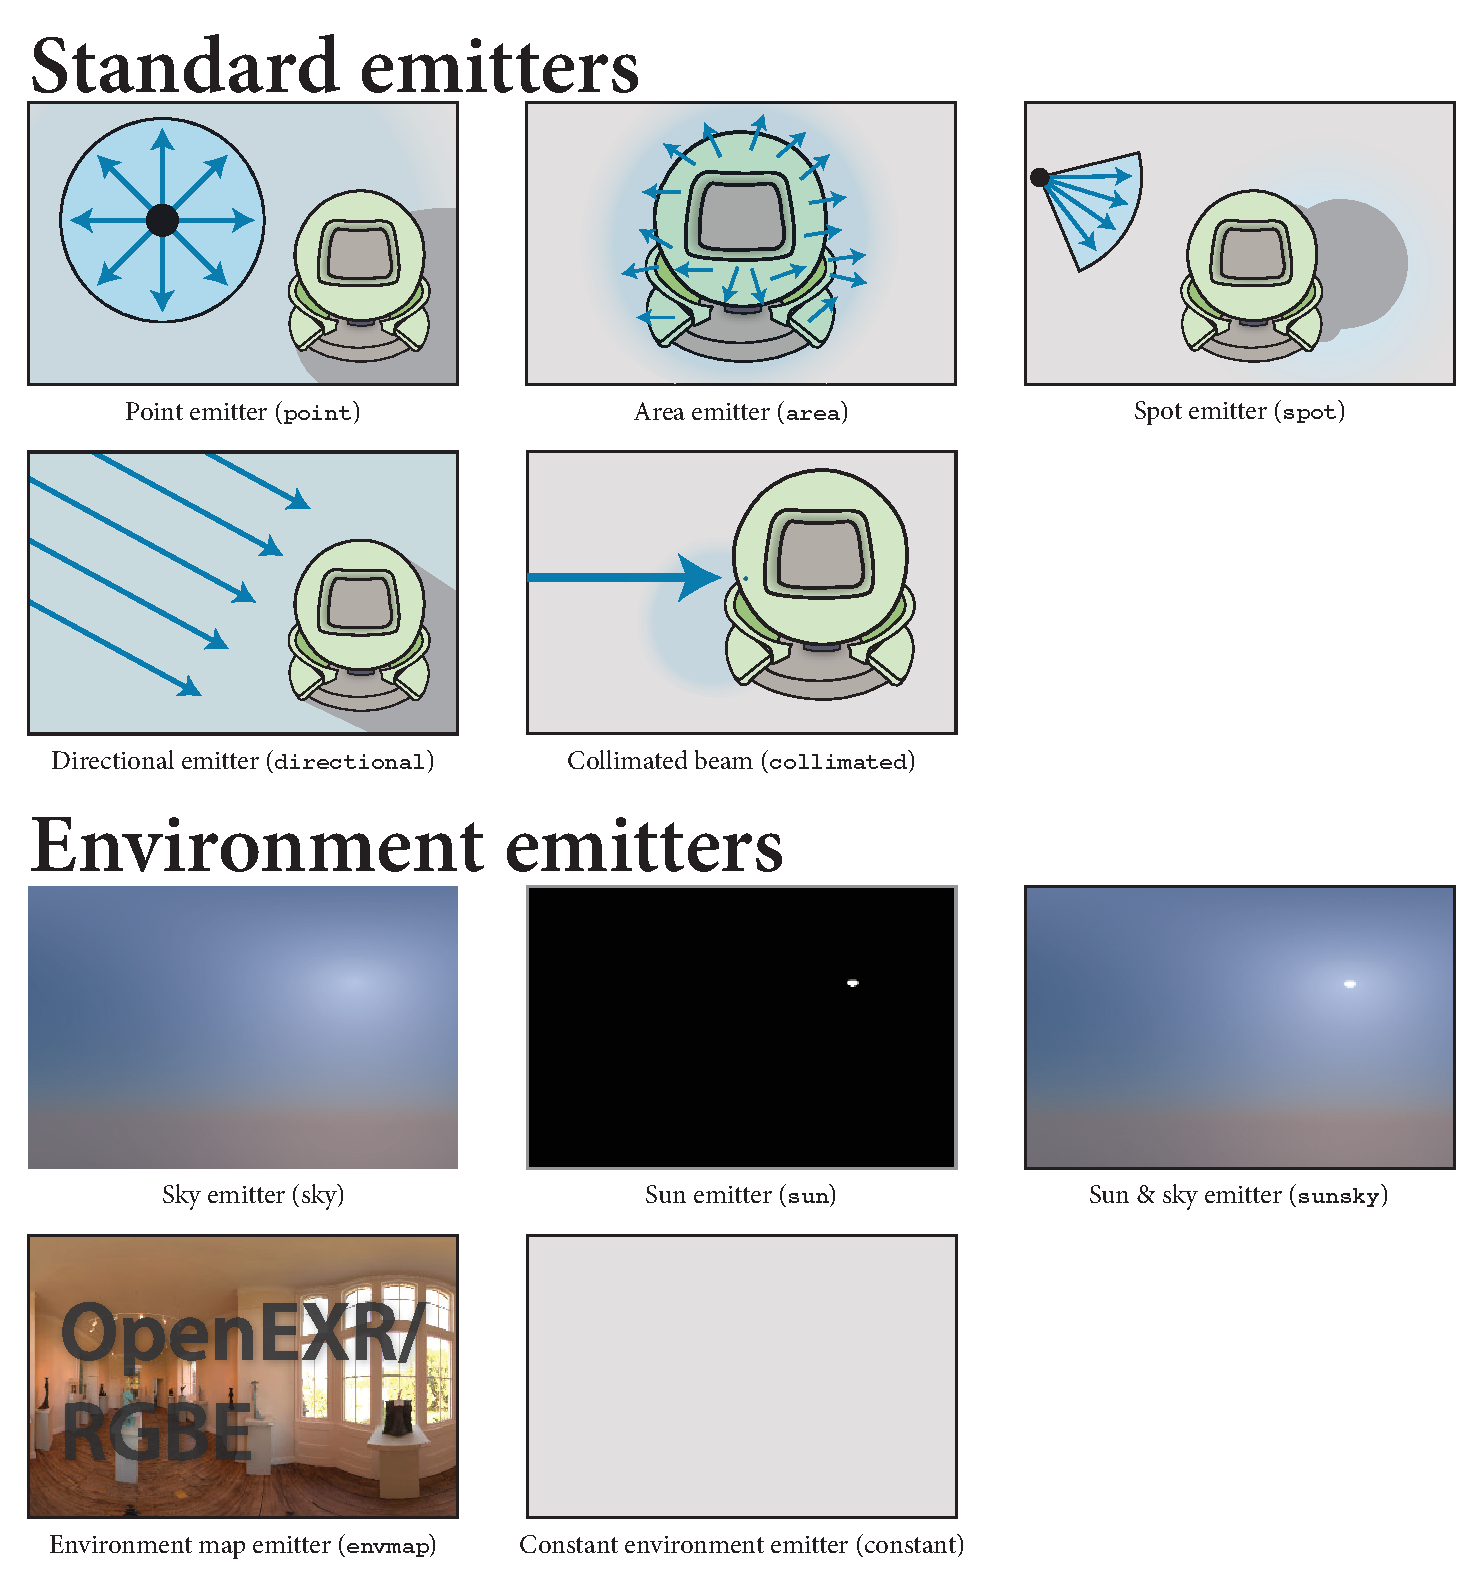
\includegraphics[width=15.5cm]{images/emitter_overview.pdf}
\caption{
    Schematic overview of the most important emitters in Mitsuba.
    The arrows indicate the directional distribution of light.
}
\end{figure}
\newpage
Generally, light sources are specified as children of the \code{<scene>} element; for instance,
the following snippet instantiates a point light emitter that illuminates a sphere.
\begin{xml}
<scene version=$\MtsVer$>
	<emitter type="point">
		<spectrum name="intensity" value="1"/>
		<point name="position" x="0" y="0" z="-2"/>
	</emitter>
	<shape type="sphere"/>
</scene>
\end{xml}
An exception to this are \emph{area lights}, which turn a geometric object into a light source.
These are specified as children of the corresponding \code{<shape>} element.
\begin{xml}
<scene version=$\MtsVer$>
	<shape type="sphere">
		<emitter type="area">
			<spectrum name="radiance" value="1"/>
		</emitter>
	</shape>
</scene>
\end{xml}
Note the parameter names used to specify the light source power, which reflect
the different associated physical units.
